\label{chap:results}

In this chapter we will cover the results obtained with this gateway platform.

\begin{figure}[ht] \centering
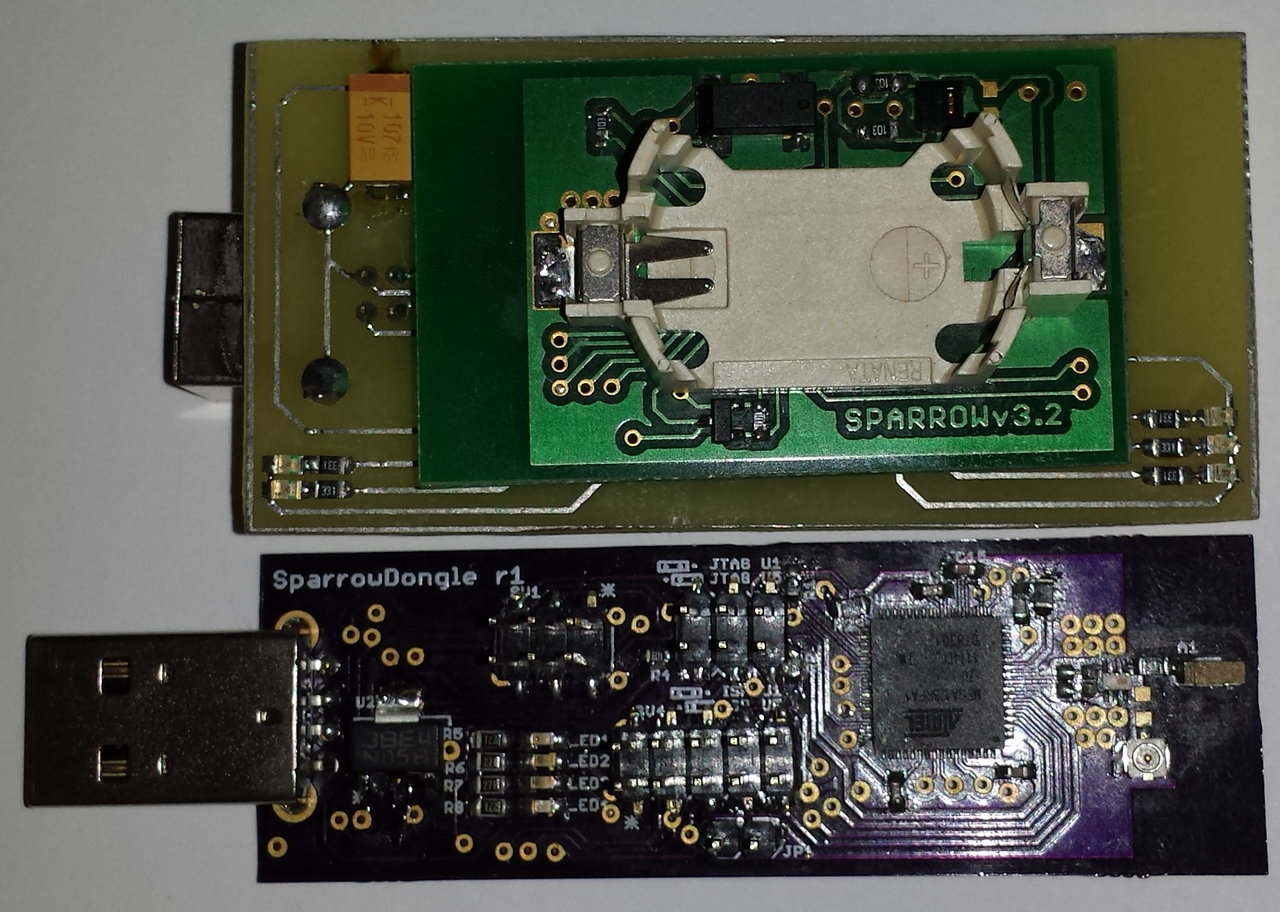
\includegraphics[width=0.45\textwidth]{img/sparrow.jpg} \caption{SparrowV3.2 and SparrowDongle} \end{figure}

 
\subsection{Performance}

The platform can detect multiple wireless sensors and offer real time feedback. 
The delay is small, but it can vary directly proportional with the distance 
between the drone and the phone and between the drone and sensor. Usually this 
delay can start from 10 ms and pass 150ms for high distance connection. Also,
thanks to the transmission speed of 250kbps, big data is transfered in under 3 
seconds. After the transfer is complete, it can be uploaded to the remote sever 
for further processing.
 

\subsection{Hardware}

The dongle fits tightly between the body and the shell of the drone. This can 
represent a future problem on different types of drones where a smaller dongle 
may be required. 

Because the drone has a powerful arm processor, it can do most of the processing 
required to fly and to detect and collect data from nodes. By using this approach,
even when the drone loses connection to the mobile phone, it can hover on its own 
until the connection is reestablished.


\subsection{Software configurations}

The software solution is very versatile. It can be ported on every platform and 
programing language that supports sockets, also the dongle and the nodes ca be
reprogrammed following the application specifications in which they are used.
 
At the moment, the following modes of operation are available, but more are to follow:

\begin{itemize}

\item \textit{Node discovery}: Nodes can be discovered and located easily when the drone
is in proximity.

\item \textit{Data server}: This mode allows the drone to save the data and to
be accessed even when the drone's power supply is removed or it is not flying 
or connected to any node 

\item \textit{Debug Tool}: The drone can have a list of nodes that are located on it's flight 
course and can detect the node that is causing the network not to function properly.

 \end{itemize}

 

